\chapter{Các không gian con, toán tử chiếu và phép đo dưới dạng vướng víu}

Định lý Bell để lại hai câu hỏi chưa được giải đáp. Vướng víu còn lại thế nào khi một thành viên của cặp bị nhiễu loạn, hấp thụ hoặc đo? Và chính xác thì điều gì biến một tương tác thông thường thành phép đo? Lối đi đến câu trả lời bắt đầu từ đại số tuyến tính sơ cấp. Các tính chất là những không gian con, xác suất là giá trị kỳ vọng của các toán tử chiếu, còn thiết bị đo là một hệ lượng tử khác mà vật thể trở nên vướng víu với nó.

\section{Động cơ mở đầu: vướng víu, tính địa phương và phép đo}

Giả sử một trạng thái singlet đã được tách thành hai phần ở xa nhau và một phần được đo. Thuyết trường lượng tử có nhất thiết phải mô tả một trao đổi ảo giữa chúng không? Ở phía xa không xảy ra điều gì có thể phát hiện được, và cũng không có thông điệp hữu ích nào đến được đó. Ta có thể dùng một từ trường để quay cục bộ một spin, làm thay đổi dạng cụ thể của trạng thái chung, trong khi mức độ vướng víu vẫn giữ nguyên dưới phép toán cục bộ ấy. Các thước đo định lượng mức độ vướng víu sẽ được bàn đến sau; điểm cần lưu ý trước mắt là hai hệ đã không còn tương tác với nhau thì không thể làm thay đổi mức vướng víu chung chỉ bằng một phép toán giới hạn ở một phía.

\begin{classroomqa}
\lecturetimestamp{00:00:22}
\audiencequestion{Phép đo một thành viên của trạng thái singlet cách nhau kiểu không-thời gian có đòi hỏi trao đổi ảo nào đó với thành viên kia không?}
\lecturerresponse{Không có trao đổi nào có thể phát hiện được ở phía bên kia. Một phép toán cục bộ có thể làm quay một thừa số và thay đổi dạng biểu diễn của trạng thái chung, nhưng tự nó không thể gửi thông điệp hay làm thay đổi mức vướng víu chung giữa hai phía cách biệt.}
\end{classroomqa}

Điều đó buộc ta phải mở rộng khái niệm về đối tác của một hệ. Nếu một thành viên của cặp vướng víu rơi vào lỗ đen, thành viên kia không vì thế mà hết vướng víu; nó trở nên vướng víu với các bậc tự do của lỗ đen, rồi sau khi lỗ đen bốc hơi, với bức xạ phát ra. Không cần đến lỗ đen mới có được ý tưởng tương tự. Hãy thả một thành viên của cặp vướng víu vào bồn tắm và để nó hòa trộn dữ dội với nước. Dù bản sắc riêng của nó có thể bị mất trong trạng thái nhiều hạt, hạt ở xa vẫn vướng víu với toàn bộ bồn tắm, rồi cuối cùng với hơi nước thoát ra.

Đây không chỉ là câu chuyện về sự tồn tại dai dẳng. Đây còn là câu chuyện về tính thuận nghịch. Nếu tương tác có thể tạo ra vướng víu, thì về nguyên tắc, tương tác cũng có thể đảo ngược nó. Có thể khử vướng víu, nhưng chỉ khi các hệ tiếp xúc trở lại và tương tác với nhau. Điều gì có thể xảy ra theo một chiều thì cũng có thể xảy ra theo chiều ngược lại.

\begin{classroomqa}
\lecturetimestamp{00:04:45}
\audiencequestion{Nếu đo cả hai spin của một cặp vướng víu, các electron có còn vướng víu với nhau không? Chỉ một phép đo đã đủ làm chúng hết vướng víu chưa?}
\lecturerresponse{Các phép đo có thể loại bỏ vướng víu giữa chúng, và chỉ một phép đo cũng có thể là đủ. Để hiểu ý nghĩa của khẳng định đó thay vì chỉ đơn thuần viện dẫn sự sụp đổ, ta cần mô tả phép quan sát như một tương tác giữa hệ và thiết bị ghi nhận.}
\end{classroomqa}

Câu hỏi ấy xác định mục tiêu: liên hệ phép quan sát, sự sụp đổ của gói sóng và vướng víu. Tuy nhiên, trước khi tiếp cận vấn đề, ta cần trình bày rõ hơn về các không gian con và toán tử chiếu, chỉ dùng những công cụ cần thiết cho lập luận.

\section{Số chiều, sự phụ thuộc tuyến tính và cơ sở trực chuẩn}

Vì vậy, tạm thời ta chỉ xét các không gian vectơ hữu hạn chiều được trang bị bra, ket và tích trong. Susskind bắt đầu với những khái niệm sơ đẳng nhất có thể. Ông không định nghĩa số chiều bằng cách đếm các thành phần của một vectơ cột. Thay vào đó, ông đưa ra định nghĩa trừu tượng: số chiều của một không gian vectơ là số vectơ độc lập tuyến tính lớn nhất có thể tìm được trong không gian ấy.

Vì thế, một tập hợp \(\{|v_i\rangle\}\) là độc lập tuyến tính khi hệ thức
\begin{equation}
\sum_i c_i |v_i\rangle = 0
\end{equation}
đòi hỏi mọi hệ số \(c_i\) đều bằng không. Nói cách khác, không vectơ nào có thể được viết thành tổ hợp tuyến tính của các vectơ còn lại.

Ở đây, điều cốt yếu là tính trực giao không đồng nghĩa với tính độc lập. Trong không gian ba chiều, có thể có ba vectơ không trực giao với nhau nhưng vẫn độc lập tuyến tính. Điều quan trọng là một vectơ trong số đó có thể được tạo thành từ hai vectơ còn lại hay không. Ngược lại, trong một mặt phẳng hai chiều, bất kỳ vectơ thứ ba nào nằm trong mặt phẳng ấy cũng phải phụ thuộc tuyến tính vào hai vectơ đầu.

\begin{figure}[htbp]
\centering
\includegraphics[width=0.56\textwidth]{lecture_06_figure_02.png}
\caption{Ba vectơ được vẽ trên bảng. Bài giảng dùng hình phác này để phân biệt khái niệm trực giao với khái niệm độc lập tuyến tính, rồi nhấn mạnh rằng trong một mặt phẳng, vectơ thứ ba phụ thuộc tuyến tính vào hai vectơ đầu.}
\lectureframe{00:09:35}
\end{figure}

\begin{figure}[htbp]
\centering
\begin{tikzpicture}[scale=1.2]
\draw[->] (0,0) -- (2.3,0);
\draw[->] (0,0) -- (2.0,2.0);
\draw[->] (0.35,0.95) -- (1.05,1.45);
\fill (0,0) circle (1.2pt);
\end{tikzpicture}
\caption{Bản dựng lại tối giản hình phác trên bảng. Chỉ riêng khung hình không xác định được chính xác quan hệ giữa các hệ số; điểm hình học ở đây là trong mặt phẳng hai chiều, vectơ thứ ba không độc lập.}
\end{figure}

Đó là điểm cốt yếu của hình phác. Nếu không gian có hai chiều, số vectơ độc lập tuyến tính tối đa là hai. Nếu không gian có ba chiều, số đó là ba. Tổng quát hơn, nếu không gian có số chiều \(d\), thì với một tích trong, ta có thể tìm được \(d\) vectơ đơn vị trực giao đôi một và sinh ra không gian ấy. Đó là các vectơ cơ sở. Susskind nói rõ rằng ông sẽ không chứng minh định lý này ở đây. Ông chỉ cần kết luận: một khi có cơ sở như vậy, mọi vectơ trong không gian đều có thể khai triển theo cơ sở đó.

\begin{classroomqa}
\lecturetimestamp{00:10:58}
\audiencequestion{Số bậc tự do trong không gian có bằng số chiều của không gian trạng thái không?}
\lecturerresponse{Không. Một hạt chuyển động trong căn phòng có ba tọa độ không gian nhưng lại có vô số trạng thái lượng tử trực giao đôi một. Số chiều của không gian cấu hình và số chiều của không gian Hilbert là hai khái niệm khác nhau; các ví dụ hữu hạn chiều chỉ được dùng để làm sáng tỏ lập luận.}
\end{classroomqa}

\section{Khai triển theo cơ sở, tích dyad và phép phân giải toán tử đơn vị}

Giờ hãy chọn một cơ sở trực chuẩn \(\{|n\rangle\}\), với \(n=1,\dots,d\). Phần trình bày trên bảng ở đoạn này đặc biệt rõ ràng và súc tích:

\begin{figure}[htbp]
\centering
\includegraphics[width=0.62\textwidth]{lecture_06_figure_03.png}
\caption{Cơ sở trực chuẩn và khai triển của một trạng thái bất kỳ.}
\lectureframe{00:14:15}
\end{figure}

Ta viết
\begin{align}
\langle m|n\rangle &= \delta_{mn}, \\
|\psi\rangle &= \sum_n a_n |n\rangle.
\end{align}
Ở đây, \(\delta_{mn}\) là delta Kronecker: nó bằng \(1\) khi \(m=n\) và bằng \(0\) trong các trường hợp còn lại.

\paragraph{Phép suy dẫn có lời giải.} Các hệ số được xác định bằng cách chiếu lên cơ sở. Nhân bên trái với \(\langle m|\):
\begin{align}
\langle m|\psi\rangle
  &= \sum_n a_n \langle m|n\rangle \\
  &= \sum_n a_n \delta_{mn} \\
  &= a_m.
\end{align}
Vậy các hệ số đơn giản là
\begin{equation}
a_m = \langle m|\psi\rangle.
\end{equation}
Hệ số là một số phức thông thường, nên có thể đặt ở hai phía của ket mà không làm thay đổi điều gì.

Thay hệ số trở lại khai triển, ta được
\begin{equation}
|\psi\rangle = \sum_n |n\rangle \langle n|\psi\rangle.
\end{equation}
Điều này gợi ý rằng đối tượng \(|n\rangle\langle n|\), và tổng quát hơn là \(|a\rangle\langle b|\), nên được hiểu là một toán tử. Đó chính là bước tiếp theo. Một tích dyad tác dụng theo cách sau:
\begin{equation}
\bigl(|a\rangle\langle b|\bigr)|\psi\rangle = \langle b|\psi\rangle\,|a\rangle.
\end{equation}
Bra trích ra một số phức; ket cung cấp phương hướng tương ứng. Đây là lối tiếp cận giản dị của Susskind để đi từ vectơ đến toán tử.

Giờ hãy đọc khai triển vừa rồi dưới dạng toán tử. Vì
\begin{equation}
|\psi\rangle = \left(\sum_n |n\rangle\langle n|\right)|\psi\rangle
\end{equation}
đúng với mọi \(|\psi\rangle\), nên toán tử trong ngoặc phải là toán tử đơn vị:
\begin{equation}
\sum_n |n\rangle\langle n| = I.
\end{equation}
Đây là phép phân giải toán tử đơn vị.

\begin{figure}[htbp]
\centering
\includegraphics[width=0.60\textwidth]{lecture_06_figure_07.png}
\caption{Phép phân giải toán tử đơn vị hoàn chỉnh trên bảng.}
\lectureframe{00:18:30}
\end{figure}

\begin{classroomqa}
\lecturetimestamp{00:18:39}
\audiencequestion{Các vectơ trong phép phân giải toán tử đơn vị có nhất thiết phải tạo thành một cơ sở không?}
\lecturerresponse{Có. Phép suy dẫn dựa trên cả điều kiện chuẩn hóa lẫn tính trực giao đôi một, và tổng phải chạy trên một cơ sở đầy đủ. Một tập vectơ tùy ý không phân giải được toán tử đơn vị.}
\end{classroomqa}

Bản thân toán tử đơn vị là toán tử chiếu lên toàn bộ không gian. Mọi vectơ đều là vectơ riêng của \(I\), và mọi giá trị riêng đều bằng \(+1\).

\begin{classroomqa}
\lecturetimestamp{00:19:14}
\audiencequestion{Phép phân giải toán tử đơn vị có nói rằng mọi vectơ đều có giá trị riêng bằng một không?}
\lecturerresponse{Có, đối với toán tử đơn vị. Đây là trường hợp đặc biệt, trong đó mọi vectơ đều là vectơ riêng của nó và \(I|\psi\rangle=|\psi\rangle\) với mọi trạng thái.}
\end{classroomqa}

\section{Các tính chất dưới dạng không gian con và toán tử chiếu}

Với những công cụ ấy, bài giảng đưa ra sự điều chỉnh khái niệm then chốt. Một tính chất như \(k=\lambda\) nói chung không phải là một vectơ đơn lẻ. Đó là cả một không gian con.

Cho \(k\) là một đại lượng quan sát Hermite và giả sử
\begin{equation}
k|A\rangle = \lambda |A\rangle, \qquad
k|B\rangle = \lambda |B\rangle,
\end{equation}
trong đó \(|A\rangle\) và \(|B\rangle\) độc lập tuyến tính. Khi ấy, mọi tổ hợp tuyến tính đều có cùng giá trị riêng:
\begin{align}
k\bigl(\alpha|A\rangle+\beta|B\rangle\bigr)
  &= \alpha k|A\rangle + \beta k|B\rangle \\
  &= \alpha \lambda |A\rangle + \beta \lambda |B\rangle \\
  &= \lambda\bigl(\alpha|A\rangle+\beta|B\rangle\bigr).
\end{align}
Vậy không gian riêng ứng với \(\lambda\) đóng dưới phép cộng và phép nhân với vô hướng. Nó là một không gian vectơ con.

Ví dụ cụ thể đầu tiên trong bài giảng là hệ gồm hai spin. Các trạng thái
\begin{equation}
|ud\rangle,\qquad |uu\rangle
\end{equation}
có giá trị khác nhau của spin thứ hai, nhưng cùng giá trị của spin thứ nhất: trong cả hai trường hợp, spin thứ nhất đều hướng lên. Vì thế, chúng sinh ra không gian con trong đó \(\sigma_3=+1\) đối với spin thứ nhất.

\begin{figure}[htbp]
\centering
\includegraphics[width=0.46\textwidth]{lecture_06_figure_04.png}
\caption{Hai trạng thái của hệ hai spin có spin thứ nhất hướng lên.}
\lectureframe{00:23:27}
\end{figure}

Điểm cần giữ lại là: một tính chất không nhất thiết tương ứng với một trạng thái duy nhất. Đó là cả một tập hợp các trạng thái có cùng giá trị riêng.

Để tránh nhầm lẫn ký hiệu xuất hiện thoáng qua trên bảng, ta sẽ dùng chữ in hoa \(A,B,\dots\) cho các vectơ riêng cụ thể, còn chữ thường \(a,b,\dots\) làm chỉ số tổng chạy trên một cơ sở trực chuẩn của không gian riêng con. Nếu \(\{|a\rangle\}\) là một cơ sở như vậy của không gian con \(k=\lambda\), thì toán tử chiếu lên không gian con đó là
\begin{equation}
\Pi_{k=\lambda}=\sum_a |a\rangle\langle a|.
\end{equation}
Đây chính là toán tử đơn vị bị giới hạn vào không gian con. Nếu \(|\psi\rangle\) đã nằm trong không gian con ấy, phép chiếu trả lại nó nguyên vẹn. Nếu \(|\psi\rangle\) có một phần nằm ngoài không gian con, phép chiếu loại bỏ phần trực giao bên ngoài và chỉ giữ lại thành phần bên trong.

\section{Tiên đề xác suất, các tính chất tương thích và phần ôn lại về Bell}

Khi đã diễn giải lại các tính chất thành không gian con, tiên đề xác suất có dạng rõ ràng nhất. Nếu \(|\psi\rangle\) đã được chuẩn hóa, thì xác suất để nó có tính chất \(k=\lambda\) là
\begin{equation}
P(k=\lambda)=\langle\psi|\Pi_{k=\lambda}|\psi\rangle.
\end{equation}

\begin{figure}[htbp]
\centering
\includegraphics[width=0.58\textwidth]{lecture_06_figure_05.png}
\caption{Toán tử chiếu lên không gian riêng con ứng với \(k=\lambda\). Cách trình bày trên bảng đã chuẩn bị cho bước tiếp theo: đặt toán tử chiếu vào giữa \(\langle\psi|\) và \(|\psi\rangle\).}
\lectureframe{00:31:09}
\end{figure}

Thay dạng dyad của toán tử chiếu vào biểu thức:
\begin{align}
P(k=\lambda)
  &= \left\langle \psi \left| \sum_a |a\rangle\langle a| \right| \psi \right\rangle \\
  &= \sum_a \langle\psi|a\rangle\langle a|\psi\rangle \\
  &= \sum_a |\langle a|\psi\rangle|^2.
\end{align}
Đây chính là cách diễn giải trong bài giảng: xác suất tổng cộng của tính chất bằng tổng xác suất của tất cả các khả năng trực giao mà tính chất đó có thể xảy ra.

Đối với trường hợp spin thứ nhất hướng lên trong hệ hai spin, không gian con liên quan được sinh bởi \(|uu\rangle\) và \(|ud\rangle\), nên
\begin{equation}
\Pi_{\sigma_3=+1}=|uu\rangle\langle uu|+|ud\rangle\langle ud|.
\end{equation}
Theo cách viết tắt trong bài giảng, biểu thức này cũng được viết là
\begin{equation}
\Pi_{\sigma_3=+1}=\frac{1+\sigma_3}{2},
\end{equation}
trong đó toán tử đơn vị tác dụng lên spin thứ hai được lược bỏ.

\begin{classroomqa}
\lecturetimestamp{00:33:04}
\audiencequestion{Đại lượng quan sát, tính chất và toán tử chiếu khác nhau thế nào?}
\lecturerresponse{Đại lượng quan sát là toán tử Hermite \(k\). Tính chất \(k=\lambda\) được biểu diễn bởi không gian riêng của nó, nghĩa là nếu đo \(k\) thì chắc chắn thu được \(\lambda\). Toán tử chiếu \(\Pi_{k=\lambda}\) cô lập không gian riêng ấy, còn giá trị kỳ vọng của nó cho biết xác suất tính chất đó hiện diện.}
\end{classroomqa}

\begin{classroomqa}
\lecturetimestamp{00:34:07}
\audiencequestion{Các vectơ riêng suy biến \(A\) và \(B\) có nhất thiết đã trực giao với nhau không, và chúng có tạo thành cơ sở của toàn bộ không gian không?}
\lecturerresponse{Các vectơ riêng ban đầu không nhất thiết trực giao với nhau, nhưng luôn có thể chọn một cơ sở trực chuẩn bên trong không gian riêng con của chúng. Cơ sở này chỉ là cơ sở của không gian con ấy; để sinh ra toàn bộ không gian, cần thêm các phương trực giao. Chiếu lên từng vectơ cơ sở của không gian con rồi cộng lại sẽ cho phép chiếu lên toàn bộ không gian con.}
\end{classroomqa}

\begin{classroomqa}
\lecturetimestamp{00:35:33}
\audiencequestion{Ký hiệu \(a\) trong \(k|A\rangle=\lambda|A\rangle\) có nghĩa giống với \(a\) được lấy tổng trong toán tử chiếu không?}
\lecturerresponse{Không. Ký hiệu thứ nhất chỉ một vectơ riêng cụ thể, còn chỉ số dưới dấu tổng chạy qua mọi vectơ trong một cơ sở trực chuẩn của không gian riêng con. Dùng ký hiệu khác nhau giúp tránh nhầm một nhãn cố định với chỉ số lấy tổng.}
\end{classroomqa}

\begin{classroomqa}
\lecturetimestamp{00:37:15}
\audiencequestion{Các tích trong trong công thức toán tử chiếu là xác suất hay biên độ xác suất?}
\lecturerresponse{Mỗi \(\langle a|\psi\rangle\) là một biên độ. Nhân nó với số phức liên hợp sẽ cho một xác suất; cộng các xác suất ấy trên những cách trực giao để thực hiện \(k=\lambda\) sẽ cho xác suất tổng cộng của tính chất.}
\end{classroomqa}

Tiếp đó, bài giảng đặt câu hỏi làm thế nào kết hợp các tính chất. Giả sử ta có hai tính chất tương thích, được biểu diễn bởi các toán tử chiếu giao hoán \(P_k\) và \(P_\ell\). Theo cách diễn đạt trong bài giảng, mệnh đề AND được biểu diễn bằng tích:
\begin{equation}
\Pi_{k=\lambda\,\wedge\,\ell=\mu}=P_kP_\ell=P_\ell P_k.
\end{equation}
Lập luận rất đơn giản. \(P_k|\psi\rangle\) nằm trong không gian con \(k=\lambda\). Vì các toán tử giao hoán nên \(P_\ell P_k|\psi\rangle=P_kP_\ell|\psi\rangle\), do đó cùng vectơ ấy cũng nằm trong không gian con \(\ell=\mu\). Vậy tích các toán tử chiếu lên tính chất đồng thời. Xác suất tương ứng là
\begin{equation}
P(k=\lambda,\ell=\mu)=\langle\psi|P_kP_\ell|\psi\rangle.
\end{equation}

Bước đầu tiên trong lập luận ấy đáng được trình bày riêng. Với trạng thái bất kỳ,
\begin{equation}
k\bigl(P_k|\psi\rangle\bigr)=\lambda P_k|\psi\rangle,
\end{equation}
cho nên \(P_k|\psi\rangle\) nằm trong không gian riêng \(k=\lambda\). Nếu \(P_k\) và \(P_\ell\) giao hoán, ta có thể viết tích với một trong hai toán tử chiếu đặt bên trái; vì vậy vectơ thuộc cả hai không gian con.

\begin{figure}[htbp]
\centering
\includegraphics[width=0.44\textwidth]{lecture_06_figure_06.png}
\caption{Trạng thái sau phép chiếu được biểu diễn thành một vectơ trong không gian riêng con.}
\lectureframe{00:41:57}
\end{figure}

\begin{figure}[htbp]
\centering
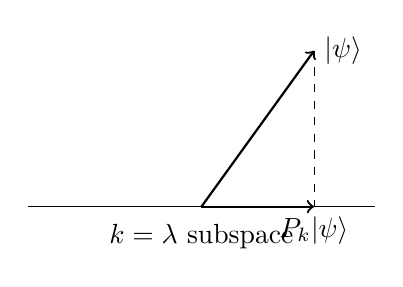
\begin{tikzpicture}[scale=1.1]
\draw (-2,0) -- (2,0);
\draw[->,thick] (0,0) -- (1.3,1.8) node[right] {$|\psi\rangle$};
\draw[dashed] (1.3,1.8) -- (1.3,0);
\draw[->,thick] (0,0) -- (1.3,0) node[below] {$P_k|\psi\rangle$};
\node at (0,-0.35) {$k=\lambda$ subspace};
\end{tikzpicture}
\caption{Chiếu một vectơ bất kỳ vào không gian riêng con \(k=\lambda\).}
\end{figure}

\begin{figure}[htbp]
\centering
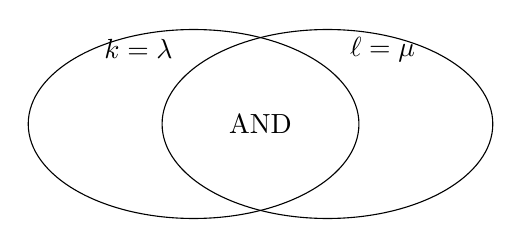
\begin{tikzpicture}[scale=1.0]
\draw (0,0) ellipse (2.1 and 1.2);
\draw (1.7,0) ellipse (2.1 and 1.2);
\node at (-0.7,0.95) {$k=\lambda$};
\node at (2.4,0.95) {$\ell=\mu$};
\node at (0.85,0) {AND};
\end{tikzpicture}
\caption{Hình dựng lại minh họa hai không gian con giao nhau, làm nền tảng cho mệnh đề AND đối với các toán tử chiếu giao hoán.}
\end{figure}

\begin{figure}[htbp]
\centering
\includegraphics[width=0.66\textwidth]{lecture_06_figure_08.png}
\caption{Lập luận trên bảng cho thấy các toán tử chiếu giao hoán chọn ra không gian riêng đồng thời.}
\lectureframe{00:45:20}
\end{figure}

\begin{classroomqa}
\lecturetimestamp{00:44:42}
\audiencequestion{Tính chất đồng thời có giống với phép giao trong logic cổ điển không?}
\lecturerresponse{Có. Với các toán tử chiếu giao hoán, \(P_kP_\ell\) chiếu lên giao của hai không gian riêng. Nếu giao đó chỉ chứa vectơ không, thì không có trạng thái khác không nào có cả hai tính chất.}
\end{classroomqa}

Để đầy đủ, toán tử chiếu lên không gian con OR tương thích là
\begin{equation}
P_{k\lor\ell}=P_k+P_\ell-P_kP_\ell .
\end{equation}
Khi hai khả năng loại trừ lẫn nhau, \(P_kP_\ell=0\) và biểu thức rút gọn thành tổng \(P_k+P_\ell\). Phép trừ này là thiết yếu khi hai không gian con có phần giao, vì nếu không thì phần giao sẽ bị tính hai lần.

Sau đó, tính tương thích được liên hệ lại với các ví dụ vật lý. Trong hệ hai spin, mọi thành phần \(\sigma_i\) của spin thứ nhất đều giao hoán với mọi thành phần \(\tau_j\) của spin thứ hai:
\begin{equation}
[\sigma_i,\tau_j]=0.
\end{equation}
Ngược lại, các thành phần khác nhau của cùng một spin không giao hoán:
\begin{equation}
[\sigma_1,\sigma_3]\neq 0.
\end{equation}
Đó là lý do ta có thể đo một thành phần của mỗi spin trong hai spin cách biệt, nhưng không thể đồng thời đo hai thành phần khác nhau của cùng một spin.

\begin{classroomqa}
\lecturetimestamp{00:46:12}
\audiencequestion{Có những ví dụ cụ thể nào về các đại lượng quan sát tương thích?}
\lecturerresponse{Mọi toán tử tác dụng lên spin thứ nhất đều giao hoán với mọi toán tử tác dụng lên spin thứ hai, vì chúng tác dụng lên các thừa số tensor khác nhau. Các thành phần vị trí \(x,y,z\) cũng là một họ tương thích. Ngược lại, hai thành phần khác nhau của cùng một spin, hoặc vị trí và động lượng liên hợp với nó, không giao hoán.}
\end{classroomqa}

\begin{classroomqa}
\lecturetimestamp{00:47:26}
\audiencequestion{Một hệ con có nhất thiết phải là một hạt khác không?}
\lecturerresponse{Không. Đó là một tập hợp bậc tự do được xác định độc lập. Các hạt khác nhau tạo thành những thừa số tensor đơn giản nhất, nhưng khi cấu trúc toán tử cho phép, ta cũng có thể xem xét riêng các bậc tự do khác nhau của cùng một hạt.}
\end{classroomqa}

\begin{classroomqa}
\lecturetimestamp{00:48:37}
\audiencequestion{Nếu nhiều toán tử trên các hệ con khác nhau giao hoán như vậy, có cặp không tương thích đơn giản nào không?}
\lecturerresponse{Hai thành phần của cùng một spin là ví dụ chuẩn: \(\sigma_1\) và \(\sigma_3\) không giao hoán, nên không thiết bị nào có thể đồng thời gán cho chúng cả hai giá trị xác định chính xác. Giao hoán tử ma trận khác không là phép kiểm tra đại số.}
\end{classroomqa}

Giờ Susskind quay lại định lý Bell. Ông không tính lại các phép tính của bài giảng trước. Ông xây dựng lại lập luận bằng ngôn ngữ mới. Bất đẳng thức cổ điển, viết dưới dạng xác suất, là
\begin{equation}
P(A\wedge \neg B)+P(B\wedge \neg C)\ge P(A\wedge \neg C).
\end{equation}
Đây là một định lý của logic tập hợp cổ điển, không phải của cơ học lượng tử. Trong trạng thái singlet, các spin ngược chiều nhau dọc theo mọi trục chung, nên có thể thay mệnh đề NOT đối với spin thứ nhất bằng mệnh đề khẳng định tương ứng đối với spin thứ hai. Nhờ đó, ta có thể viết lại bất đẳng thức thành một mệnh đề về các tính chất chung của hệ hai spin.

Lược bỏ các toán tử đơn vị trên những thừa số không bị tác động, các toán tử chiếu cho tính chất đơn xuất hiện trong bài giảng là
\begin{equation}
\frac{1+\sigma_3}{2},\qquad
\frac{1+\frac{\tau_1+\tau_3}{\sqrt2}}{2},\qquad
\frac{1+\frac{\sigma_1+\sigma_3}{\sqrt2}}{2},\qquad
\frac{1+\tau_1}{2}.
\end{equation}
Vì vậy, ba toán tử chiếu chung liên quan là
\begin{align}
\Pi_1 &= \frac{1+\sigma_3}{2}\,\frac{1+\frac{\tau_1+\tau_3}{\sqrt2}}{2}, \\
\Pi_2 &= \frac{1+\frac{\sigma_1+\sigma_3}{\sqrt2}}{2}\,\frac{1+\tau_1}{2}, \\
\Pi_3 &= \frac{1+\sigma_3}{2}\,\frac{1+\tau_1}{2}.
\end{align}

\begin{figure}[htbp]
\centering
\includegraphics[width=0.68\textwidth]{lecture_06_figure_09.png}
\caption{Ba lựa chọn bộ phân tích được viết thành tích của các toán tử chiếu một spin.}
\lectureframe{01:01:45}
\end{figure}

Bài giảng dùng dạng quen thuộc, chưa chuẩn hóa, của trạng thái singlet trên bảng:
\begin{equation}
|\Psi_{\mathrm{singlet}}\rangle \propto |ud\rangle-|du\rangle.
\end{equation}
Ký hiệu tỉ lệ là đủ ở đây. Điều quan trọng đối với lập luận là chính trạng thái, đặc biệt là dấu tương đối, chứ không phải hệ số chuẩn hóa chung. Tính \(\langle \Pi_1\rangle+\langle \Pi_2\rangle\) đối với \(\langle \Pi_3\rangle\) trong trạng thái singlet cho kết quả vi phạm thu được ở bài giảng trước. Kết luận quan trọng là điều Susskind nhấn mạnh bằng lời: không thể ngụy trang cơ học lượng tử thành lý thuyết tập hợp cổ điển.

\begin{classroomqa}
\lecturetimestamp{00:52:31}
\audiencequestion{Nếu spin hướng lên và spin hướng xuống trực giao với nhau, dấu trừ có nghĩa là một ket bằng số đối của ket kia không?}
\lecturerresponse{Không. \(|u\rangle\) và \(|d\rangle\) là hai vectơ trực giao khác nhau. Dấu tương đối thuộc về một chồng chập như \(|ud\rangle-|du\rangle\) và có thể làm thay đổi các tính chất vật lý của nó; chỉ dấu chung nhân với toàn bộ trạng thái mới không có ý nghĩa.}
\end{classroomqa}

\begin{classroomqa}
\lecturetimestamp{00:53:06}
\audiencequestion{Bất đẳng thức Bell có bị vi phạm với mọi trạng thái lượng tử và mọi lựa chọn tính chất không?}
\lecturerresponse{Không. Nhiều trạng thái và nhiều lựa chọn trục thỏa mãn một bất đẳng thức Bell cụ thể. Việc có vi phạm hay không phụ thuộc cả vào trạng thái lẫn các đại lượng quan sát được chọn. Thay đổi các góc trung gian và góc cuối sẽ làm thay đổi khả năng phép kiểm tra này bộc lộ các tương quan phi cổ điển.}
\end{classroomqa}

\begin{classroomqa}
\lecturetimestamp{01:02:47}
\audiencequestion{Có thể kết luận điều gì khi một trạng thái cụ thể vi phạm, hoặc tình cờ thỏa mãn, bất đẳng thức Bell này?}
\lecturerresponse{Việc vi phạm chứng minh rằng các thống kê quan sát được không thể xuất phát từ logic tập hợp cổ điển dùng trong phép suy dẫn. Việc thỏa mãn một bất đẳng thức được chọn không tự nó chứng tỏ trạng thái là cổ điển, vì một lựa chọn tính chất khác có thể cho thấy sự vi phạm.}
\end{classroomqa}

\section{Tính địa phương sau Bell}

Phép tính toán tử chiếu không chỉ là trò chơi ký hiệu. Hãy hình dung việc chuẩn bị lặp đi lặp lại các cặp tương quan ở trạng thái cơ bản singlet, tách hai thành viên ra, rồi chia tập hợp được chuẩn bị đồng nhất thành ba nhóm lớn. Nhóm thứ nhất đo các thiết lập \(0^\circ\) và \(45^\circ\), nhóm thứ hai đo các thiết lập \(45^\circ\) và \(90^\circ\), còn nhóm thứ ba đo các thiết lập \(0^\circ\) và \(90^\circ\). Tần suất trong ba nhóm cho phép ước lượng ba xác suất trong bất đẳng thức.

\begin{classroomqa}
\lecturetimestamp{01:04:30}
\audiencequestion{Bố trí thí nghiệm nào trong phòng thí nghiệm tương ứng với ba xác suất Bell?}
\lecturerresponse{Một nguồn tạo ra nhiều cặp vướng víu được chuẩn bị giống hệt nhau rồi gửi hai thành viên đến các bộ phân tích cách biệt. Chia các cặp thành ba tập hợp và dùng cặp hướng bộ phân tích tương ứng cho mỗi tập hợp. Đếm các kết quả chung sẽ ước lượng từng xác suất. Có thể dùng trường để tách một hạt mang điện và phản hạt của nó; trong các thí nghiệm Bell thực tế, người ta thường dùng photon hơn.}
\end{classroomqa}

\begin{classroomqa}
\lecturetimestamp{01:08:00}
\audiencequestion{Chứng minh bằng tập hợp cổ điển dùng một tập hợp hạt. Làm thế nào ba tập hợp được đo riêng rẽ có thể kiểm tra chứng minh ấy?}
\lecturerresponse{Bất đẳng thức là một mệnh đề về xác suất cũng như về số đếm. Nếu cả ba mẫu đều được lấy theo cùng một quy trình chuẩn bị, tần suất tương đối của chúng sẽ ước lượng ba phân bố xác suất của cùng một tập hợp chung. Giả thiết không thể thiếu là việc chuẩn bị đồng nhất.}
\end{classroomqa}

Phần ôn lại định lý Bell dẫn thẳng đến nỗi băn khoăn về mặt vật lý vẫn còn trong phòng. Nếu các tương quan là có thật, tại sao không thể dùng chúng để gửi tín hiệu?

\begin{classroomqa}
\lecturetimestamp{01:09:41}
\audiencequestion{Tại sao không thể dùng các tương quan vướng víu để gửi thông điệp nhanh hơn ánh sáng?}
\lecturerresponse{Ở mỗi phía, người ta vẫn chỉ thấy một chuỗi ngẫu nhiên không thể kiểm soát. Tương quan chỉ lộ rõ khi hai bản ghi được so sánh qua một kênh cổ điển thông thường. Tuy nhiên, một phép kiểm tra Bell có tính quyết định được bố trí sao cho các lựa chọn và phép phát hiện diễn ra theo cách không tín hiệu ánh sáng nào có thể truyền từ phía này sang phía kia kịp thời; nhờ đó loại trừ cơ chế truyền thông tin cục bộ tạo ra các thống kê chung.}
\end{classroomqa}

Nếu có đủ thời gian để tín hiệu ánh sáng truyền giữa các thiết bị, bản thân một tương quan không mâu thuẫn với thuyết tương đối; ta có thể chỉ vừa phát hiện ra một ảnh hưởng thông thường mà trước đó không nhận thấy. Thí nghiệm dứt khoát loại bỏ lối thoát ấy. Theo cách diễn đạt của Bell, một mô hình biến ẩn tái tạo được các tương quan phải là phi địa phương, nhưng sự phụ thuộc phi địa phương không đồng nghĩa với một thông điệp siêu quang có thể điều khiển.

\begin{classroomqa}
\lecturetimestamp{01:12:18}
\audiencequestion{Bảo toàn mômen động lượng có thiết yếu đối với lập luận này không?}
\lecturerresponse{Không. Spin là một mô hình hai trạng thái tiện dụng, chứ không phải thành phần bất khả thay thế. Bất kỳ cặp hệ hai mức nào có trạng thái vướng víu cần thiết và các cơ sở đo thay thế đều có thể thể hiện cùng cấu trúc logic.}
\end{classroomqa}

Phần thảo luận này chưa khép lại bài giảng; nó dọn đường cho bước chuyển tiếp theo. Bell cho ta thấy cơ học lượng tử không phải logic cổ điển, nhưng câu hỏi tiếp theo lại khác. Xét về mặt vận hành và toán học, phép đo là gì, và nó tham gia vào câu chuyện về giao thoa như thế nào?

\section{Thí nghiệm hai khe với số trạng thái hữu hạn, giao thoa và phép đo dưới dạng vướng víu}

Giờ bài giảng chuyển sang một mô hình khác. Susskind xét thí nghiệm hai khe, nhưng lập tức đơn giản hóa nó thành một bài toán có số trạng thái hữu hạn để có thể dùng cùng bộ công cụ không gian vectơ mà không cần đến toàn bộ lý thuyết sóng liên tục. Thậm chí, ông nói đại ý rằng đây vẫn là thí nghiệm hai khe, chỉ được giản lược xuống một tập nhỏ các trạng thái cơ sở.

Có một trạng thái nguồn \(|0\rangle\), hai trạng thái khe \(|1\rangle\) và \(|-1\rangle\), cùng một tập các trạng thái màn \(|n\rangle\). Các trạng thái \(|n\rangle\) này trực chuẩn vì những vị trí khác nhau trên màn là những cấu hình khác nhau. Trong bài giảng, người ta chủ ý không theo dõi chính xác điều kiện chuẩn hóa ở đây. Tính đơn nhất được để lại bàn sau. Ở giai đoạn này, điều quan trọng là tính tuyến tính.

\begin{figure}[htbp]
\centering
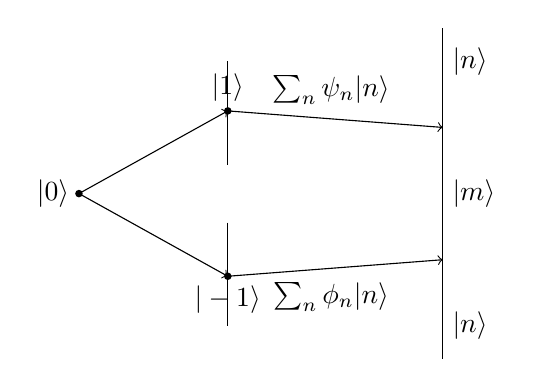
\begin{tikzpicture}[scale=1.05]
\fill (0,0) circle (1.3pt);
\node[left] at (0,0) {$|0\rangle$};

\draw (1.8,1.6) -- (1.8,0.35);
\draw (1.8,-0.35) -- (1.8,-1.6);
\fill (1.8,1) circle (1.3pt);
\fill (1.8,-1) circle (1.3pt);
\node[above] at (1.8,1) {$|1\rangle$};
\node[below] at (1.8,-1) {$|-1\rangle$};

\draw (4.4,2.0) -- (4.4,-2.0);
\node[right] at (4.4,1.6) {$|n\rangle$};
\node[right] at (4.4,0.0) {$|m\rangle$};
\node[right] at (4.4,-1.6) {$|n\rangle$};

\draw[->] (0,0) -- (1.8,1);
\draw[->] (0,0) -- (1.8,-1);
\draw[->] (1.8,1) -- (4.4,0.8);
\draw[->] (1.8,-1) -- (4.4,-0.8);

\node at (3.05,1.25) {$\sum_n \psi_n |n\rangle$};
\node at (3.05,-1.25) {$\sum_n \phi_n |n\rangle$};
\end{tikzpicture}
\caption{Phiên bản hữu hạn trạng thái của thí nghiệm hai khe: trạng thái nguồn \(|0\rangle\), hai trạng thái khe \(|1\rangle\) và \(|-1\rangle\), cùng cơ sở trên màn \(|n\rangle\).}
\end{figure}

\begin{figure}[htbp]
\centering
\includegraphics[width=0.68\textwidth]{lecture_06_figure_10.png}
\caption{Mạng vị trí hữu hạn bên cạnh quy tắc tiến hóa tuyến tính \(A\to A'\), \(B\to B'\).}
\lectureframe{01:18:00}
\end{figure}

Do tính đối xứng, trạng thái nguồn tiến hóa thành chồng chập có biên độ bằng nhau của hai trạng thái khe:
\begin{equation}
|0\rangle \longrightarrow |1\rangle+|-1\rangle.
\end{equation}
Giờ cho trạng thái khe trên tiến hóa thành
\begin{equation}
|1\rangle \longrightarrow \sum_n \psi_n |n\rangle,
\end{equation}
và trạng thái khe dưới tiến hóa thành
\begin{equation}
|-1\rangle \longrightarrow \sum_n \phi_n |n\rangle.
\end{equation}
Ở đây, các mũi tên chỉ sự tiến hóa theo thời gian, chứ không biểu thị hai trạng thái bằng nhau tại cùng một thời điểm. Theo tính tuyến tính,
\begin{equation}
|1\rangle+|-1\rangle \longrightarrow \sum_n (\psi_n+\phi_n)|n\rangle.
\end{equation}
Đó là quy tắc then chốt. Các biên độ cộng với nhau trước khi lập xác suất.

\begin{classroomqa}
\lecturetimestamp{01:21:59}
\audiencequestion{Làm thế nào trạng thái ở khe \(|1\rangle\) có thể biến đổi thành các trạng thái cũng được gắn nhãn bằng số nguyên \(n\)? Các ket này có ở cùng một vị trí và cùng một thời điểm không?}
\lecturerresponse{Các nhãn chỉ những lát cắt thời gian khác nhau. \(|1\rangle\) biểu thị electron ở khe phía trên, còn các \(|n\rangle\) bên phải biểu thị những vị trí có thể có về sau trên màn. Mũi tên chỉ sự tiến hóa theo thời gian, chứ không phải sự bằng nhau giữa các cấu hình đồng thời.}
\end{classroomqa}

\begin{classroomqa}
\lecturetimestamp{01:25:30}
\audiencequestion{Các biên độ có cần được chuẩn hóa không, và chúng có đơn vị vật lý không?}
\lecturerresponse{Một quá trình tiến hóa đầy đủ phải bảo toàn xác suất toàn phần; đó là tính unita. Ở đây, hệ số chuẩn hóa chung được lược bỏ vì điều quan trọng chỉ là sự cộng và triệt tiêu của các biên độ đường đi. Có thể khôi phục mọi hệ số tỉ lệ khi chuẩn hóa trạng thái.}
\end{classroomqa}

Vì vậy, xác suất electron đến vị trí \(m\) trên màn là
\begin{align}
P_m &= |\psi_m+\phi_m|^2 \\
    &= |\psi_m|^2 + |\phi_m|^2 + \psi_m^*\phi_m + \phi_m^*\psi_m.
\end{align}
Hai số hạng đầu là kết quả mà lập luận cổ điển sẽ đưa ra. Hai số hạng cuối là các số hạng giao thoa.

\begin{figure}[htbp]
\centering
\includegraphics[width=0.68\textwidth]{lecture_06_figure_11.png}
\caption{Biên độ tại màn và khai triển xác suất thành bốn số hạng được ghi trên bảng.}
\lectureframe{01:29:20}
\end{figure}

Tại điểm đối xứng trên màn, gọi là \(m=0\), tính đối xứng gợi ý rằng \(\psi_0=\phi_0\). Khi đó
\begin{equation}
P_0 = |\psi_0+\phi_0|^2 = |2\psi_0|^2 = 4|\psi_0|^2.
\end{equation}
Khi mở cả hai khe, xác suất tại điểm đó gấp bốn lần xác suất khi chỉ mở một khe, chứ không phải gấp đôi. Đây là giao thoa tăng cường.

Bây giờ thêm độ lệch pha sao cho \(\phi_0=-\psi_0\). Khi đó
\begin{equation}
P_0 = |\psi_0-\psi_0|^2 = 0.
\end{equation}
Từng khe riêng lẻ đều cho phép electron đến điểm đó, nhưng mở đồng thời cả hai khe có thể khiến electron không thể đến đó. Đây là giao thoa triệt tiêu. Susskind nhấn mạnh rõ điều này kỳ lạ đến mức nào: theo ông, nó kỳ lạ chẳng kém gì hiện tượng Bell.

\begin{classroomqa}
\lecturetimestamp{01:33:14}
\audiencequestion{Điều gì xảy ra nếu chỉ thay đổi bộ dịch pha hoặc lựa chọn khe sau khi electron đã đang bay? Khe còn lại có cần thời gian để biết về thay đổi đó không?}
\lecturerresponse{Câu trả lời phụ thuộc vào bố trí không-thời gian cụ thể và việc electron có đi qua phần thiết bị đã thay đổi hay không. Cơ học lượng tử mô tả sự tiến hóa của trạng thái qua bố trí thực tế; xác suất vẫn được tính bằng cách cộng các biên độ thích hợp. Muốn đánh giá các khẳng định về tính địa phương trong một đề xuất lựa chọn trễ, cần mô tả đề xuất đó thật rõ ràng.}
\end{classroomqa}

Bây giờ ta đưa thiết bị vào mô hình. Có thêm một hệ hai trạng thái, là spin ban đầu ở trạng thái \(|d\rangle\). Nếu electron đi qua khe trên, spin đó lật thành \(|u\rangle\). Nếu electron đi qua khe dưới, spin giữ nguyên. Trạng thái ban đầu của hệ kết hợp là \(|0,d\rangle\), và quy tắc cập nhật thứ nhất trở thành
\begin{equation}
|0,d\rangle \longrightarrow |1,u\rangle + |-1,d\rangle.
\end{equation}
Một dòng đó diễn đạt trọn vẹn ý nghĩa của phép đo trong bài giảng. Vị trí của electron đã trở nên vướng víu với bản ghi được lưu trong thiết bị.

\begin{figure}[htbp]
\centering
\includegraphics[width=0.66\textwidth]{lecture_06_figure_12.png}
\caption{Spin của máy dò tương quan các bản ghi spin lên và xuống với hai khả năng đi qua khe.}
\lectureframe{01:44:10}
\end{figure}

\begin{classroomqa}
\lecturetimestamp{01:40:20}
\audiencequestion{Có cần đặt máy dò ở cả hai khe không?}
\lecturerresponse{Chỉ cần một máy dò đáng tin cậy. Nếu máy dò ghi nhận electron đi qua khe trên, bản ghi không đổi sẽ cho biết electron đi theo khả năng khe dưới, với điều kiện mọi electron truyền qua đều phải đi qua một trong hai khe. Có thể dùng máy dò thứ hai, nhưng như vậy chỉ thêm một hệ con mà không làm thay đổi nguyên lý.}
\end{classroomqa}

\begin{classroomqa}
\lecturetimestamp{01:40:51}
\audiencequestion{Sao không nói electron đi qua cả hai khe?}
\lecturerresponse{Khi không có bản ghi đường đi, trạng thái là một chồng chập kết hợp và không thể xác định hồi tố electron đã đi theo đường nào. Khi phép đo xác định đường đi được thực hiện đầy đủ, thiết bị ghi lại một trong hai khả năng ở mỗi lần chạy. Đại lượng tồn tại xuyên suốt cả hai khả năng là biên độ trạng thái, chứ không phải hai quỹ đạo electron riêng biệt được quan sát độc lập.}
\end{classroomqa}

\begin{figure}[htbp]
\centering
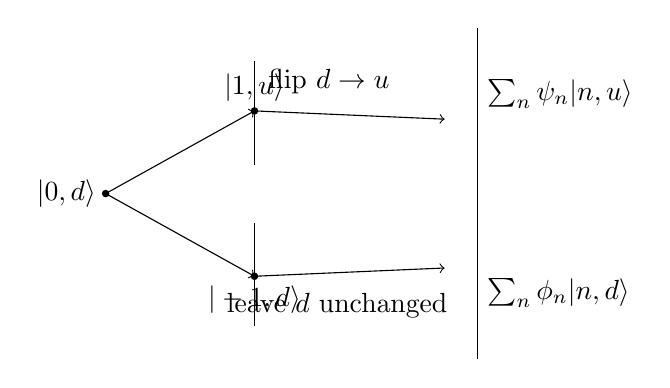
\begin{tikzpicture}[scale=1.05]
\fill (0,0) circle (1.3pt);
\node[left] at (0,0) {$|0,d\rangle$};

\draw (1.8,1.6) -- (1.8,0.35);
\draw (1.8,-0.35) -- (1.8,-1.6);
\fill (1.8,1) circle (1.3pt);
\fill (1.8,-1) circle (1.3pt);
\node[above] at (1.8,1) {$|1,u\rangle$};
\node[below] at (1.8,-1) {$|-1,d\rangle$};

\draw (4.5,2.0) -- (4.5,-2.0);
\node[right] at (4.5,1.2) {$\sum_n \psi_n |n,u\rangle$};
\node[right] at (4.5,-1.2) {$\sum_n \phi_n |n,d\rangle$};

\draw[->] (0,0) -- (1.8,1);
\draw[->] (0,0) -- (1.8,-1);
\draw[->] (1.8,1) -- (4.1,0.9);
\draw[->] (1.8,-1) -- (4.1,-0.9);

\node at (2.7,1.35) {flip \(d\to u\)};
\node at (2.8,-1.35) {leave \(d\) unchanged};
\end{tikzpicture}
\caption{Phép đo dưới dạng vướng víu với spin của máy dò. Đường đi phía trên làm lật spin của thiết bị; đường đi phía dưới giữ nguyên spin đó.}
\end{figure}

Giả sử, như trong bài giảng, spin không chịu tác động nào khác trong quá trình electron bay đến màn. Khi đó
\begin{align}
|1,u\rangle &\longrightarrow \sum_n \psi_n |n,u\rangle, \\
|-1,d\rangle &\longrightarrow \sum_n \phi_n |n,d\rangle.
\end{align}
Do đó, trạng thái cuối cùng khi mở cả hai khe là
\begin{equation}
|\Psi_{\mathrm{final}}\rangle
  = \sum_n \psi_n |n,u\rangle + \sum_n \phi_n |n,d\rangle.
\end{equation}
Đây không phải là chồng chập các trạng thái chỉ của riêng một electron. Đây là trạng thái vướng víu giữa electron và thiết bị.

\begin{figure}[htbp]
\centering
\includegraphics[width=0.68\textwidth]{lecture_06_figure_13.png}
\caption{Hai biên độ đường đi đến màn cùng với các bản ghi trực giao của thiết bị.}
\lectureframe{01:47:35}
\end{figure}

Cách đơn giản nhất để tính xác suất electron đến vị trí \(m\) là dùng toán tử chiếu lên vị trí đó trong hệ con electron:
\begin{equation}
\Pi_m = |m\rangle\langle m|\otimes I_{\mathrm{spin}}.
\end{equation}
Áp dụng \(\Pi_m\) lên trạng thái cuối cùng, ta được
\begin{equation}
\Pi_m |\Psi_{\mathrm{final}}\rangle
= |m\rangle\bigl(\psi_m|u\rangle+\phi_m|d\rangle\bigr).
\end{equation}
Vậy xác suất electron đến \(m\) là
\begin{align}
P_m
  &= \langle \Psi_{\mathrm{final}}|\Pi_m|\Psi_{\mathrm{final}}\rangle \\
  &= \bigl(\psi_m^*\langle u|+\phi_m^*\langle d|\bigr)
     \bigl(\psi_m|u\rangle+\phi_m|d\rangle\bigr) \\
  &= |\psi_m|^2 + |\phi_m|^2
     + \psi_m^*\phi_m\langle u|d\rangle
     + \phi_m^*\psi_m\langle d|u\rangle.
\end{align}
Nhưng các trạng thái bản ghi trực giao với nhau:
\begin{equation}
\langle u|d\rangle=0.
\end{equation}
Do đó, các số hạng chéo triệt tiêu:
\begin{equation}
P_m = |\psi_m|^2 + |\phi_m|^2.
\end{equation}
Đó là điểm mấu chốt về mặt toán học của bài giảng. Một khi thông tin đường đi được ghi lại, giao thoa biến mất và xác suất cộng với nhau theo cách cổ điển.

\begin{classroomqa}
\lecturetimestamp{01:49:09}
\audiencequestion{Chồng chập \(|1\rangle+|-1\rangle\) khác trạng thái \(|1,u\rangle+|-1,d\rangle\) ở điểm nào?}
\lecturerresponse{Trường hợp thứ nhất nói về một hệ ở trong tổ hợp tuyến tính của hai vị trí; không có hệ nào khác để nó có thể vướng víu cùng. Trường hợp thứ hai nói về hai hệ, trong đó đường đi tương quan với spin của máy dò. Đọc trạng thái spin khi đó sẽ cho biết thông tin về đường đi.}
\end{classroomqa}

\section{Các bản ghi môi trường và phép đo một phần}

Máy dò được chế tạo có chủ đích không phải là vật duy nhất có thể ghi lại đường đi. Một nguyên tử gần khe, khí dư, bề mặt nhiệt hoặc bất kỳ bậc tự do nào khác đều có thể trở nên tương quan với đường đi. Nếu trạng thái cuối của nó là \(|E_1\rangle\) và \(|E_2\rangle\), trạng thái đường đi có dạng
\begin{equation}
|\Psi\rangle
=\sum_n\left(\psi_n|n\rangle|E_1\rangle
+\phi_n|n\rangle|E_2\rangle\right).
\end{equation}
Các số hạng giao thoa lúc này được nhân với độ chồng lấp \(\langle E_1|E_2\rangle\). Các bản ghi trực giao khiến hai đường đi có thể phân biệt hoàn toàn và xóa sạch giao thoa. Các bản ghi giống hệt nhau cho \(\langle E_1|E_2\rangle=1\) và giữ nguyên giao thoa. Độ chồng lấp ở mức trung gian tạo ra độ tương phản giao thoa một phần.

\begin{figure}[htbp]
\centering
\includegraphics[width=0.68\textwidth]{lecture_06_figure_14.png}
\caption{Các gói sóng môi trường chồng lấp và tách biệt minh họa các bản ghi đường đi một phần và đầy đủ.}
\lectureframe{01:53:40}
\end{figure}

\begin{classroomqa}
\lecturetimestamp{01:50:48}
\audiencequestion{Một nguyên tử bình thường ở gần khe có vướng víu với electron đi qua không, ngay cả khi không ai chủ ý quan sát nó?}
\lecturerresponse{Có. Từ then chốt ở đây không phải là biết, mà là tương quan vật lý. Nếu nguyên tử hoặc khí xung quanh bị nhiễu động đủ để trạng thái về sau của chúng phân biệt được đường đi, chúng sẽ ghi lại thông tin về đường đi và làm suy giảm giao thoa. Vì vậy, các thí nghiệm như thế đòi hỏi phải cách ly, làm lạnh đến nhiệt độ thấp và thường dùng các hạt tương tác yếu như photon.}
\end{classroomqa}

Làm lạnh đưa các bậc tự do của môi trường về gần trạng thái cơ bản và giảm các bản ghi ngoài ý muốn. Độ chênh năng lượng cũng có tác dụng: nếu hạt tới không thể cung cấp năng lượng kích thích tối thiểu, môi trường có thể không giữ lại được thông tin đường đi. Ngược lại, các hạt mang điện có thể gây nhiễu vật chất ở gần thông qua điện trường của chúng, khiến việc quan sát giao thoa electron đặc biệt khó khăn.

\begin{classroomqa}
\lecturetimestamp{01:54:49}
\audiencequestion{Có thể thực sự thu được hình giao thoa bằng các electron đơn lẻ không?}
\lecturerresponse{Mỗi electron chỉ tạo ra một vết va chạm định xứ. Cho từng hạt đi qua một lần, với khoảng cách đủ lớn để chúng không tương tác, rồi ghi nhận nhiều lần lặp lại. Phân bố tần suất tích lũy sẽ hiện ra hình giao thoa; một sự kiện riêng lẻ chỉ là một chấm nhỏ.}
\end{classroomqa}

\begin{classroomqa}
\lecturetimestamp{01:55:59}
\audiencequestion{Phép đo phá hủy hay tạo ra sự vướng víu?}
\lecturerresponse{Tương tác xác định đường đi tạo ra sự vướng víu giữa hệ và thiết bị, và sự vướng víu đó phá hủy giao thoa giữa các khả năng. Một phép đo về sau có thể làm thiết bị tương quan với một hệ khác nữa và có thể điều kiện hóa trạng thái còn lại, vì vậy cần luôn nêu rõ đang nói đến hai hệ con nào và sự giao thoa nào.}
\end{classroomqa}

\begin{classroomqa}
\lecturetimestamp{01:57:44}
\audiencequestion{Có thể làm yếu tương tác để thiết bị chỉ thu được một phần thông tin đường đi không?}
\lecturerresponse{Có. Tương tác yếu có thể chỉ làm lật máy dò với một biên độ nào đó, khiến các trạng thái bản ghi không trực giao. Khi đó, hai đường đi chỉ phân biệt được một phần và giao thoa cũng chỉ suy giảm một phần. Phép đo càng mạnh thì hai đường đi càng dễ phân biệt, sự vướng víu với bản ghi càng mạnh và độ hiện rõ của các vân giao thoa càng thấp.}
\end{classroomqa}

Vì vậy, sự sụp đổ liên quan ở đây có ý nghĩa cụ thể: đó là sự mất đi của các số hạng chéo khi thông tin đường đi đã được chuyển sang một hệ khác. Không có bản ghi thì các biên độ cộng với nhau. Khi các bản ghi phân biệt được hoàn toàn, tích vô hướng giữa chúng bằng không và các xác suất cộng với nhau. Giữa hai giới hạn đó, cường độ phép đo và độ hiện rõ của giao thoa biến thiên liên tục.
